\chapter{Konzeption}
In diesem Kapitel wird der konzeptionelle Entwurf der entwickelten Lösung detailliert beschrieben. Die Konzeption umfasst alle wesentlichen Aspekte der Systemarchitektur, der Prozessabläufe sowie der Benutzeroberflächen. Dabei war es entscheidend, sowohl die technischen Anforderungen als auch die Nutzerbedürfnisse optimal zu berücksichtigen.
\newline
Zunächst wird der Workflow des Anfrageprozesses dargestellt, um die Abfolge und Logik der einzelnen Prozessschritte zu veranschaulichen. Dies bildet die Grundlage für die spätere Implementierung der Abläufe und dient dazu, alle Beteiligten über die genauen Prozessschritte zu informieren.
\newline
Daraufhin folgt das UML-Diagramm, das die Backend-Struktur des Systems beschreibt. Das Diagramm verdeutlicht die technischen Komponenten sowie deren Beziehungen zueinander.
\newline
Schließlich werden die Mockups vorgestellt, die die geplanten Benutzeroberflächen visualisieren. Diese grafischen Entwürfe dienen als Grundlage für die spätere Implementierung der Benutzeroberfläche und helfen dabei, die Nutzerinteraktionen und das Design bereits in der frühen Phase des Projekts zu planen.
\newline
Die einzelnen Konzepte in den folgenden Unterkapiteln bieten somit einen umfassenden Überblick über die geplante Systemarchitektur, den Prozessablauf und die Benutzerführung.
\newpage
\section{Workflow}
Der dargestellte Workflow (s. Abbildung \ref{fig:Workflow}) beschreibt den vollständigen Ablauf eines Anfrageprozesses, der mehrere Phasen durchläuft, um eine effiziente und strukturierte Bearbeitung sicherzustellen. Dieser Prozess beginnt mit der Erstellung einer Anfrage und endet mit der finalen Analyse und Bewertung durch den Anfragenden.
\subsection*{Entwurfsphase (Draft)}
Der Prozess beginnt mit der Erstellung der Anfrage. In dieser Phase bereitet der Antragsteller alle relevanten Informationen vor, die für die Anfrage notwendig sind. Die Anfrage wird jedoch noch nicht an die zuständigen Personen gesendet, sondern verbleibt als Entwurf. Hier kann der Antragsteller die Anfrage noch überarbeiten, Details hinzufügen oder Anpassungen vornehmen. Der Entwurfsstatus ermöglicht es, die Anfrage zu optimieren, bevor sie offiziell eingereicht wird. Sobald der Antragsteller alle notwendigen Informationen eingetragen hat und bereit ist, die Anfrage weiterzuleiten, wird diese in den nächsten Schritt überführt.
\subsection*{Offene Phase (Open)}
Nachdem die Anfrage finalisiert wurde, wird sie aus dem Entwurfsstatus herausgesendet. In der Phase \texttt{Open}  können nun die zuständigen Mitarbeiter die Anfrage einsehen.
\newline
Der nächste Schritt im Prozess ist die Entscheidung, ob die Anfrage akzeptiert wird. Wenn die Anfrage nicht akzeptiert wird, endet der Prozess an dieser Stelle und die Anfrage wird entweder abgelehnt oder zurückgezogen. In solchen Fällen wird keine weitere Bearbeitung vorgenommen, und der Anfragende wird informiert.
\newline
Wird die Anfrage hingegen akzeptiert, erfolgt die Zuweisung einer verantwortlichen Person, die die Bearbeitung übernimmt. Dieser Schritt ist entscheidend, da die Verantwortung für den weiteren Verlauf der Anfrage klar festgelegt wird.
\subsection*{In Bearbeitung (In Progress)}
In dieser Phase wird die Anfrage aktiv bearbeitet. Die verantwortliche Person prüft zunächst die Anfrage und den damit verbundenen Arbeitsaufwand. Ein wichtiger Entscheidungspunkt in diesem Abschnitt ist, ob es noch offene Fragen gibt, die mit dem Antragsteller geklärt werden müssen. Falls Fragen bestehen, wird der Antragsteller kontaktiert, um Unklarheiten zu beseitigen und gegebenenfalls zusätzliche Informationen anzufordern.
\newline
Sobald alle notwendigen Informationen vorliegen und alle Fragen geklärt sind, beginnt die Erstellung der Analyse. Diese Analyse kann je nach Anfrageumfang und -komplexität unterschiedlich viel Zeit in Anspruch nehmen. Die Analyse ist der Kern des Bearbeitungsprozesses, da hier die eigentliche Auswertung der angeforderten Daten oder Informationen stattfindet.
\newline
Während der Analysephase ist es weiterhin möglich, dass der Antragsteller oder die verantwortliche Person Rückfragen haben oder zusätzliche Details geklärt werden müssen. Es kann notwendig sein, dass eine enge Zusammenarbeit zwischen dem Analysten und dem Antragsteller erforderlich ist, um sicherzustellen, dass die Analyse den Erwartungen entspricht.
\newline
Parallel zur Analyse wird auch eine Einigung zwischen dem Analysten und dem Antragsteller getroffen. Hierbei wird geprüft, ob beide Seiten mit dem Fortschritt und den Bedingungen der Anfrage zufrieden sind. Sollte keine Einigung erzielt werden, wird der Prozess in die abgelehnte Phase überführt.
\subsection*{Abgelehnt/Zur{\"u}ckgezogen (Rejected/Revoked)}
Falls die Einigung zwischen dem Antragsteller und dem Analysten nicht erreicht wird, oder wenn während des Prozesses festgestellt wird, dass die Anfrage nicht weiter verfolgt werden kann, wird die Anfrage in den Status \texttt{Rejected} oder \texttt{Revoked} versetzt. Dieser Status beendet den Anfrageprozess vorzeitig. Gründe für diesen Abbruch könnten unklare Anforderungen, nicht erfüllbare Bedingungen oder andere Hindernisse sein, die den Abschluss der Anfrage verhindern.
\subsection*{Abschlussphase (Done)}
Ist die Analyse abgeschlossen und alle offenen Punkte geklärt, wird die Analyse an den Antragsteller gesendet. Der Antragsteller hat nun die Möglichkeit, die fertige Analyse zu überprüfen und zu bewerten, ob die Ergebnisse seinen Erwartungen entsprechen. Diese Phase ermöglicht es dem Antragsteller, die übermittelten Informationen detailliert zu prüfen und sicherzustellen, dass alle Anforderungen erfüllt sind.
\newline
Falls der Antragsteller nach der Überprüfung zufrieden ist, wird der Prozess abgeschlossen und der Status der Anfrage auf \texttt{Done} gesetzt. Sollte der Antragsteller noch weitere Fragen oder Anliegen haben, besteht die Möglichkeit, den Analysten zu kontaktieren, um diese Punkte zu klären. Der Prozess wird erst dann als abgeschlossen betrachtet, wenn der Antragsteller vollständig zufrieden ist und alle Anliegen gelöst wurden.
\newline
In dieser finalen Phase spielt die Kommunikation zwischen dem Analysten und dem Antragsteller eine wichtige Rolle, um sicherzustellen, dass alle Erwartungen erfüllt wurden und der Prozess erfolgreich abgeschlossen werden kann.
\begin{figure}[H]
    \centering
    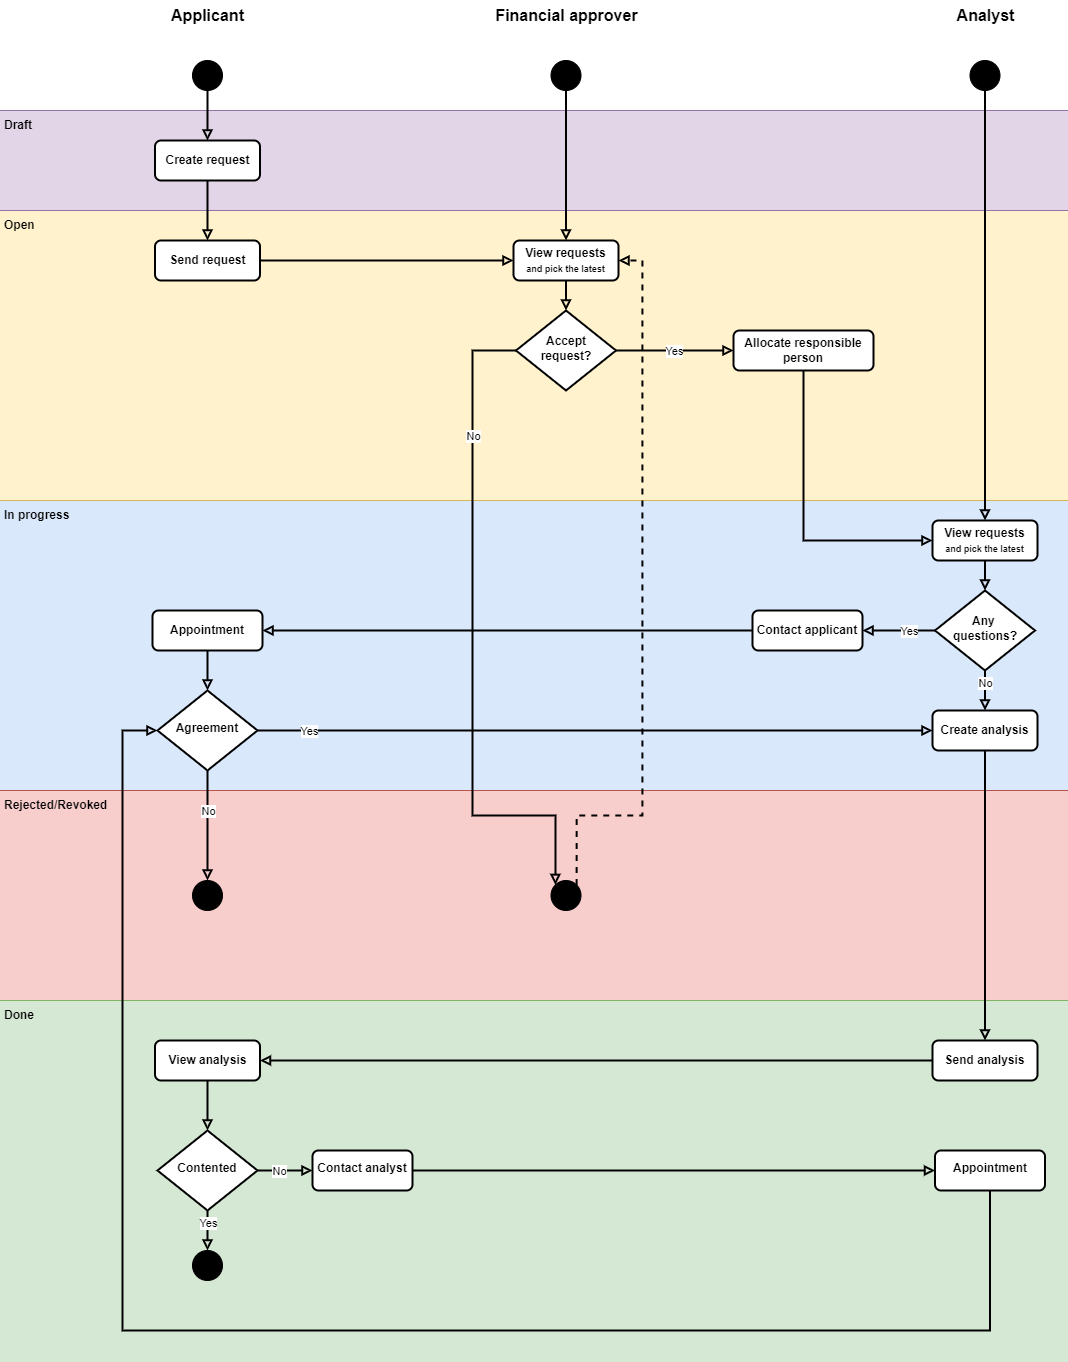
\includegraphics[scale=.4]{media/Workflow}
    \caption{Workflow}
    \label{fig:Workflow}
\end{figure}
\newpage
\section{UML-Diagramm}
Das UML-Diagramm (s. Abbildung \ref{fig:UML_Diagramm})veranschaulicht die zentrale Struktur des IAV Merida Request-Tools und modelliert die Klassen sowie deren Beziehungen im Backend. Im Zentrum steht die Klasse \texttt{Request}, die eine einzelne Anfrage repräsentiert. Diese Klasse enthält Attribute wie eine eindeutige ID, einen Titel sowie das Erstellungsdatum und enthält somit die grundlegenden Informationen der jeweiligen Anfrage.
\newline
Die Klasse \texttt{Request} ist zudem mit mehreren Enumerationen verknüpft: \texttt{State}, \texttt{Output} und \texttt{Report}. Die Enumeration \texttt{State} beschreibt den aktuellen Status der Anfrage und ermöglicht es, den Fortschritt der Anfrage nachzuvollziehen. So können Anfragen beispielsweise als \texttt{NEW}, \texttt{IN\_PROGRESS} oder \texttt{COMPLETED} markiert werden. Das Enumeration \texttt{Output} beschreibt das gewünschte Ausgabeformat der Anfrage, welches in Form von \texttt{REPORT}, \texttt{TRACES} oder \texttt{CONVERSION} erfolgen kann. Zusätzlich unterteilt die Enumeration \texttt{Report} den Bericht in verschiedene Typen, beispielsweise \texttt{STATIC\_REPORT}, \texttt{DYNAMIC\_REPORT} oder \texttt{FILE\_EXPORT}. Dabei ist zu beachten, dass jede Anfrage genau einen Status und einen spezifischen Berichtstyp haben kann.
\newline
Eine weitere zentrale Komponente im System ist die Klasse \texttt{Vehicle}. Diese beschreibt Fahrzeuge, die einer Anfrage zugeordnet werden können. Eine Anfrage kann mehrere Fahrzeuge umfassen, wobei jedes Fahrzeug genau einer Anfrage zugeordnet ist. Ein ähnliches Verhältnis besteht zwischen der Klasse \texttt{Request} und der Klasse \texttt{Fleet}. Flotten und Fahrzeuge stehen ebenfalls in einer Beziehung zueinander, sodass bei Auswahl einer bestimmten Flotte die dazugehörigen Fahrzeuge angezeigt werden.
\newline
Darüber hinaus gibt es die Klasse \texttt{BasicData}, die alle grundlegenden Informationen einer Anfrage, wie den Titel und das Ziel, speichert. Die Klasse \texttt{TimePeriod} spezifiziert die Zeitspanne, über die eine Messung oder Analyse hinweg durchgeführt wird. Um Anfragen einer bestimmten Person zuzuordnen, existiert die Klasse \texttt{Person}, in der die Eckdaten des Users gespeichert sind, der die Anfrage erstellt.
\newline
Zusammengefasst visualisiert das UML-Diagramm die Kernkomponenten des IAV Merida Request-Tools sowie deren Beziehungen. Es bietet einen klaren Überblick über die Art und Weise, wie Anfragen erfasst, verfolgt und durch Berichte sowie Ausgabeformen ergänzt werden können. Die Beziehungen zwischen den Klassen sorgen für eine flexible Verwaltung, während die verschiedenen Berichtstypen und Ausgabemöglichkeiten das System erweitern.
\begin{figure}[H]
    \centering
    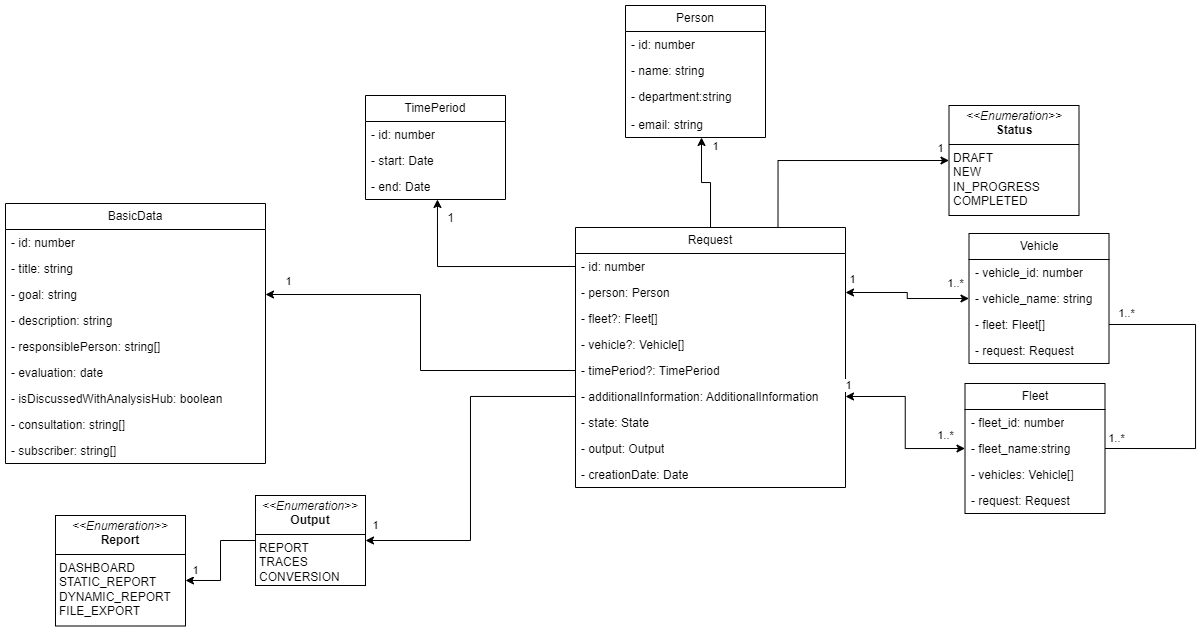
\includegraphics[angle=90, scale=.45]{media/UML_Diagramm}
    \caption{UML-Diagramm}
    \label{fig:UML_Diagramm}
\end{figure}
\label{chap:kapitel5}